\documentclass[11pt,a4paper]{report}
\usepackage[utf8]{inputenc}
\usepackage[T1]{fontenc}
\usepackage{microtype}
\usepackage[dvips]{graphicx}
\usepackage{xcolor}
\usepackage{times}
\usepackage{ragged2e}
\usepackage{titlesec}
\usepackage{wrapfig,subfigure,setspace,verbatim,cite,url,graphicx,float}
\usepackage{amsmath}
\usepackage{algorithm}
\usepackage{algpseudocode}
\usepackage{amsfonts,amssymb,calc,calrsfs,cleveref}
\usepackage[justification=centering]{caption}
\usepackage{url}
\usepackage{subfigure}
\usepackage{cleveref}

\makeatletter
\def\BState{\State\hskip-\ALG@thistlm}
\makeatother

\usepackage[
breaklinks=true,colorlinks=true,
%linkcolor=blue,urlcolor=blue,citecolor=blue,% PDF VIEW
linkcolor=black,urlcolor=black,citecolor=black,% PRINT
bookmarks=true,bookmarksopenlevel=2]{hyperref}

\usepackage{geometry}
% PDF VIEW
\geometry{total={210mm,297mm},
left=25mm,right=25mm,%
bindingoffset=0mm, top=25mm,bottom=25mm}
%PRINT
\geometry{total={210mm,297mm},
left=20mm,right=20mm,
bindingoffset=0mm, top=15mm,bottom=35mm}

\linespread{2}

\titleformat{\chapter}[display]
        {\normalfont\Large\bfseries\centering}{\chaptertitlename\ \thechapter}{0pt}{\Large\uppercase}
        
\renewcommand{\contentsname}{CONTENTS}
\renewcommand{\listfigurename}{LIST OF FIGURES}
\renewcommand{\listtablename}{LIST OF TABLES}
\renewcommand{\abstractname}{ABSTRACT}

% Make chapter titles uppercase is a pain.
% The internal chapter macros must be redefined.
\makeatletter
\renewcommand\chapter{\if@openright\cleardoublepage\else\clearpage\fi
                    \thispagestyle{plain}%
                    \global\@topnum\z@
                    \@afterindentfalse
                    \secdef\@chapter\@schapter}
\def\@chapter[#1]#2{\ifnum \c@secnumdepth >\m@ne
                       \if@mainmatter
                         \refstepcounter{chapter}%
                         \typeout{\@chapapp\space\thechapter.}%
                         \addcontentsline{toc}{chapter}%
                         {\protect\numberline{\thechapter}\texorpdfstring{\MakeUppercase{#1}}{#1}}%
                       \else
                       \addcontentsline{toc}{chapter}{\texorpdfstring{\MakeUppercase{#1}}{#1}}%
                       \fi
                    \else
                    \addcontentsline{toc}{chapter}{\texorpdfstring{\MakeUppercase{#1}}{#1}}%
                    \fi
                    \chaptermark{#1}%
                    \addtocontents{lof}{\protect\addvspace{10\p@}}%
                    \addtocontents{lot}{\protect\addvspace{10\p@}}%
                    \if@twocolumn
                      \@topnewpage[\@makechapterhead{#2}]%
                    \else
                      \@makechapterhead{#2}%
                      \@afterheading
                    \fi}
\makeatother

%%%---%%%---%%%---%%%---%%%---%%%---%%%---%%%---%%%---%%%---%%%---%%%---%%%

\begin{document}

%%%---%%%---%%%---%%%---%%%---%%%---%%%---%%%---%%%---%%%---%%%---%%%---%%%
%   TITLEPAGE
%
%   due to variety of titlepage schemes it is probably better to make titlepage manually
%
%%%---%%%---%%%---%%%---%%%---%%%---%%%---%%%---%%%---%%%---%%%---%%%---%%%
\thispagestyle{empty}

{%%%
\sffamily
\centering

{\Large 
Parallelization of Push-based System for Molecular Simulation Data Analysis with GPU
}

\vspace{1.5cm}

{
by
}
\vspace{.5cm}

{ 
Iliiazbek Akhmedov
}

\vspace{3.5cm}

A thesis submitted in partial fulfillment

of the requirements for the degree of

Master of Science in Computer Science

Department of Computer Science and Engineering

College of Engineering

University of South Florida

\vspace{3.5cm}
Major Professor:  Yicheng Tu, Ph.D.
\vspace{\fill}


\vspace{.5cm}
Date of Approval:

N/A
\vspace{\fill}

Copyright \textcopyright\space 2016, Iliiazbek Akhmedov

%%%
}%%%

\clearpage

\newgeometry{left=20mm,right=20mm,top=35mm,bottom=35mm}

\pagestyle{plain}
\centering

\textbf{DEDICATION}
\vspace{0.5cm}

\begin{flushleft}
\hspace{3em} I dedicate my thesis work to my family who have always been supporting me throughout my life. I also dedicate it to my closest friends who have shared my passion and encouraged me to explore and try my ideas in life.
\end{flushleft}

\clearpage

\pagestyle{plain}
\centering
\textbf{ACKNOWLEDGMENTS}
\vspace{0.5cm}

\begin{flushleft}
\hspace{3em} I would like to thank my major professor throughout my master thesis Dr. Yicheng Tu for his guidance and knowledge that I received through all the time I worked with him. I really appreciate his contribution and very happy that I got a chance to work with him. I as well want to thank the committee members for their support and encouragement.
\end{flushleft}

\clearpage
\restoregeometry

\linespread{1}

\tableofcontents

\addcontentsline{toc}{chapter}{\listfigurename}
\listoffigures

\addcontentsline{toc}{chapter}{\listtablename} 
\listoftables

\linespread{2}
\clearpage

\addcontentsline{toc}{chapter}{\abstractname} 
\begin{abstract}
\justify
\hspace{3em} Modern simulation systems generate big amount of data, which consequently has to be analyzed in a timely fashion. Traditional database management systems follow principle of pulling the needed data, processing it, and then returning the results. This approach is then optimized by means of caching, storing in different structures, or doing some sacrifices on precision of the results to make it faster. When it comes to the point of doing various queries that require analysis  of the whole data,  this design has the following disadvantages: considerable overhead on traditional disk random I/O framework while reading from the simulation output files and low throughput of the data that consequently results in long latency, and, if there was any indexing to optimize selections, overhead of storing those becomes too big, too. Besides it, indexing will also cause delay during write operations and since most of the queries work with the entire data sets, indexing loses its point.

There is a new approach to this problem -- Push-based System for Molecular Simulation Data Analysis for processing network of queries proposed in the previous paper and its primary steps are: i) it uses traditional scan-based I/O framework to load the data from files to the main memory and then ii) the data is pushed through a network of queries which consequently filters the data and collect all the needed information which increases efficiency and data throughput. It has a considerable advantage in analysis of molecular simulation data, because it normally involves all the data sets to be processed by the queries.

In this paper, we propose improved version of Push-based System for Molecular Simulation Data Analysis. Its major difference with the previous design is usage of GPU for the actual processing part of the data flow. Using the same scan-based I/O framework the data is pushed through the network of queries which are processed by GPU, and due to the nature of science simulation data, this gives a big advantage for processing it faster and easier (it will be explained more in later sections). In the old approach there were some custom data structures such as quad-tree for calculation of histograms to make the processing faster and those involved loss of data and some expectations from the data nature, too. In the new approach due to high performance of GPU processing and its nature, custom data structures were not even needed much, though it didn't bear any loss in precision and performance.
\end{abstract}

%%%---%%%---%%%---%%%---%%%---%%%---%%%---%%%---%%%---%%%---%%%---%%%---%%%
%%%---%%%---%%%---%%%---%%%---%%%---%%%---%%%---%%%---%%%---%%%---%%%---%%%

\chapter{Introduction}

\justify
In various sciences simulation systems take big place and often times they may be the clue for results. One of such sciences, which is primarily related to this paper, is physics. In this case, from computer engineering point of view, simulations have the following flow:

\vspace{5mm}

\begin{enumerate}
	\item initial physical properties are given to simulation software as arguments which are interpreted and provided in a language defined by the simulation software
	\item then it runs for given amount of time that can generally last from milliseconds to months or even more
	\item finally, the file generated during the simulation is analyzed to extract useful information
\end{enumerate}

\vspace{3mm}
The purpose of this paper is primarily focused on the third step, which basically involves the entire simulation data to be processed by the analysis software. It is important to underline scale of data being discussed. Molecular simulations represent systems starting from hundreds thousands of atoms and more which are tracked by frames as snapshot of specific time and can last for months. Thus, the size of data starts from couple of gigabytes up to terabytes and petabytes.

Big data processing is becoming one of the key issues with the amount of data being generated by modern systems. Eventually, this data is required to be processed on the fly, thus, analysis software should be able to handle massive data in a very short period of time. When working with huge volume of data, there are non-trivial issues arise. For example, it can take days and weeks to analyze big enough data sets, because the data cannot be simply loaded into memory, since it can get up to terabytes, thus, it has extra overhead because of traditional random access disk I/O framework to read from disk chunks by chunks. Besides it, analysis of the data can get even more complicated, since going through certain parts of the data once would not be enough, which leads to low throughput and efficiency of loaded data. One such example, the data analysis approach has polynomial complexity just for reading the data in order to come up with result, and since the data can't simply be saved in memory, it raises the overhead of disk I/O, too. Pull-based architectures in data processing engines are inefficient, since having a set of specific queries, in order to compute them all, it is needed to fetch data, filter it, and apply needed formulas. It is inefficient, since for every query the same chunk of data needs to be pulled into the memory at least the number of queries times or more in case of more complex queries.

As it has already been mentioned in the previous paper \cite{mainPaper}, one of the modern issues of analyzing massive data on the fly is social networks. "In order for a system to be able to perform analytical examination of the data produced in such streaming media, the system should have the capability of fast data access. The reason is millions of data records (tweets) produced every second. Moreover, these tweets may have different geographical origin, introducing different languages and forms and often times containing unsolicited messages, errors,
malicious content, etc. Therefore, some low level data uniformity
and cleaning on top of the data access and management issues should
be considered and possibly incorporated in the process of analytic
investigation in order to achieve relevant result".\cite{mainPaper, nature_bigdata08,nature_bigdata12,science_social10,jcs_twitter11} Another good example would be data scale of Facebook Inc. Being the largest social network, it has huge data coming in daily \cite{fbStats}. The data warehouse of Facebook is measured to be 300PB in 2014, and the daily growth is 600TB, most of the raw data is logs, which, most of the times, are used for analytics. Analytical queries involve entire data sets that will be handy for any future strategical planning in big companies, being able to observe data behavior and much more.

The primary focus and problem in this paper is scientific data analysis. Examples brought up above are real life problems that are very similar to the scientific problem that we are focusing on in terms of data sizes. Particles simulation is one of the most popular methods of analyzing certain chemical reactions, physical processes, or other behavior of different materials.
Molecular simulations (Molecular Dynamics) are applied in different fields and represent a method of analyzing physical movements of particles, atoms, and molecules in a fixed space with a given period of time, apparently with a possibility of giving initial state for each item that is involved in the process and can affect the system. These systems are most of the time N-body simulations. The number of atoms in simulations vary in hundred of thousands, particularly, we may observe two simulation systems of a collagen fiber structure and dipalmitoylphosphatidylcholine (DPPC) bi-layer lipid system consisting of 890,000 and 402,400 atoms respectively on Figure \ref{fg:collagen_dipal}. Simulation data represents number of records of physical properties such as mass, charge, velocity, coordinates, and forces for each item aggregated as frames, where each frame represents a snapshot of time, placed with a fixed time interval which may also vary depending on the simulation itself and simulation precision requirement. "Quantities measured during the simulations are analyzed to test the theoretical
model~\cite{Frenkel:api01,Landau:cup05}. In short, the MS is proven
and powerful tool for understanding the inner-workings of a
biological system, by supplying a model description of the
biophysical and biochemical processes that are being unfold at a
nanoscopic scale." \cite{mainPaper}

Scientist gives the properties to simulation software (for example, Gromacs), runs the simulations, and finally get the output file. The output file must then be analyzed to produce certain results which may help him come up with certain consensus on original theoretical model that resulted in the molecular simulation system\cite{Frenkel:api01}. Gromacs is simulation software tool that helps scientist to run the actual simulation. It is a molecular dynamics package primarily designed for biomolecular systems such as proteins and lipids. \cite{Gromacs-online}. Besides the fact that it helps to generate the output files for the simulations, apparently it also helps to analyze the data itself, but the original problem is that it is not as optimized as it can be in order to analyze the data. Gromacs follows approach of pull-based design, which means that for any given query (e.g. total mass or total charge, which are very similar type of 1-body queries without sophisticated selection) it will pull data separately and generate addition overhead wasting disk read I/O in order to come up with the result just for a single query. As it has been proposed in the previous paper, in order to remedy such issues, the push-based design does exactly the opposite, where instead of loading the data on demand for each query, the queries are batched into a network, then the entire dataset is loaded chunk by chunk pushing it through the network which has its internal relationships and dependencies amonth the queries. In this case, since scientific simulation data is run once with specific physical properties, it is never modified, thus, on continuation, it will only append, which means that the processing can also be run on appended frames. \cite{mainPaper}
This type of approach has already been revised by other systems \cite {DataPath,Volcano,Qpipe} as of reusing loaded data through queries produced \cite {Candea,PredictablePerformance,CooperativeScans}.

In this paper, we are incorporating parallelization into the processing part of the proposed design by means of CUDA programming language for GPU. Since storage of the simulation data is very expensive, it might come to the point of analyzing the data on the fly (meaning running the simulation and analyzing it at the same time in a streaming manner), which leads to a problem of optimizing the processing part of the design proposed in the previous paper, because time spent on generating data should be tried to conceal the time spent on the processing part by means of overlapping or simply running it in a quick manner. We will talk about this in details as well in further sections.

\begin{figure}
 \centerline{ 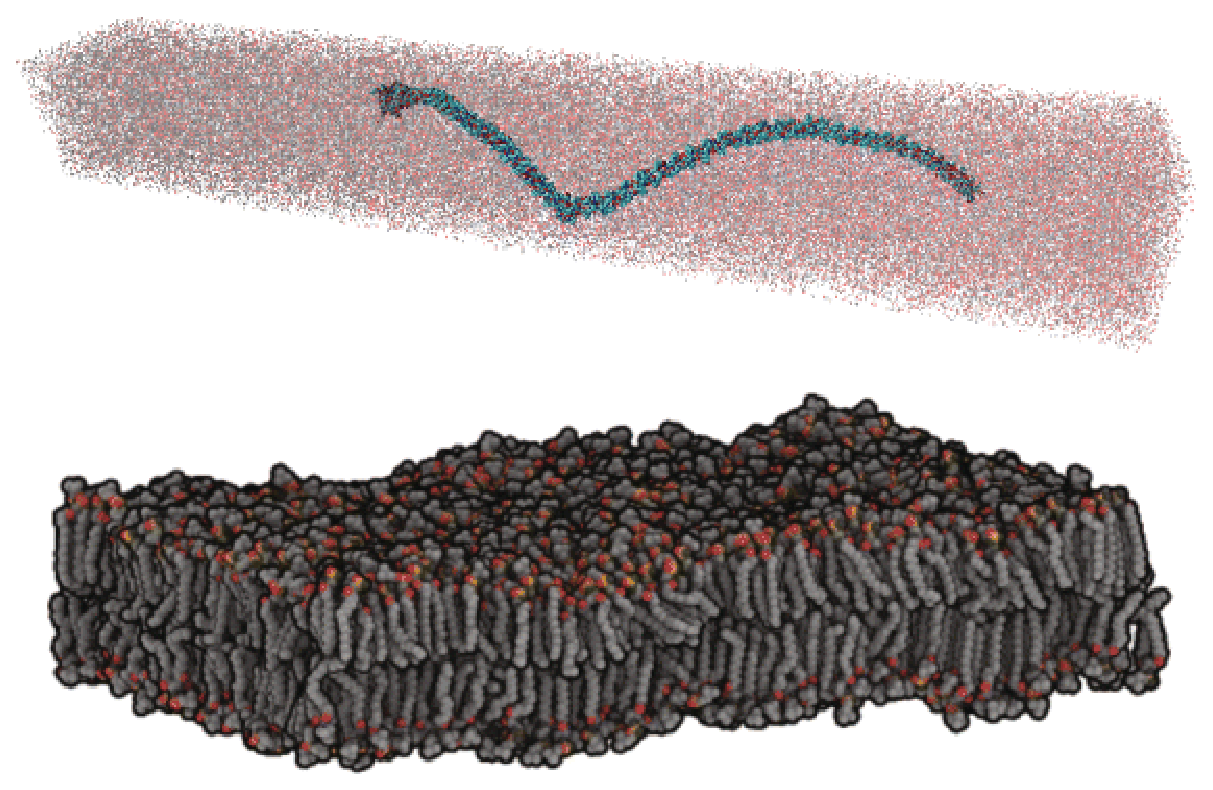
\includegraphics[width=0.5\columnwidth]{images/sample_snapshot_of_simulation.eps} }
 \caption{ Snapshots of two MS systems with 890,000 atoms with 402,400 atoms}
 \label{fg:collagen_dipal}
\end{figure}


\section{Problem Statement}
Simulation software systems, in general, follow the same methodology of running and storing simulation data. The simulation software system examples are: Gromacs \cite{GROMACS4}, VMD\cite{VMD}, MDAnalysis~\cite{MDAnalysis}, Wordom~\cite{wordom}, MD-TRACKS~\cite{MDtracks}, SimulaidOne~\cite{Simulaid}, Charmm~\cite{CHARMM}. In the type of simulations brought up as examples above, the flow of the data is the following. Once the simulation is run, the output files are contained as trajectory files with descriptors (they contain information about space dimensions, number of atoms and frames, etc.) that can be easily transposed into simple flat files containing the physical properties atom by atom, frame by frame, which are consequently read and processed by the proposed push-based system. Since we have certain amount of queries needed to be run on given simulation data, generating high I/O traffic followed by design of pull-based system is not considerable. The approach proposed in the previous paper is very good in terms of performance in comparison with the original pull-based system\cite{mainPaper}. As you can see on Figure \ref{fg:sample_estimation_old_paper}, it gets up to over 100 times of speedup which is quite crucial, if we think about days of computations. The problem is still that some of the queries processed by those means are still improvable, especially taking into consideration the fact that in the used previous works for calculation of 2-body functions, which take the biggest time for processing~\cite{ytu:icde09, EDBT12}, we might have some error bounds, which might be unacceptable for certain simulation analysis where sacrifice on loss of data is unbearable. Besides it, although we might have huge performance boost on specific data structure as density map, we still have certain expectation from data nature (such as its uniformity), thus, it makes sense to have desire to simplify the processing and still having pure computation based on any values, considering that the queries should be available to be pre-programmed by user in a separate module of the code. All the benchmarks will be done in comparison with already push-based system versus push-based system with GPU improvements. We think that it is  not fair to compare pull-based against GPU push-based approach, since the goal of the paper is to demonstrate capabilities of GPU approach that can beat simple sequential push-based system.

\begin{figure}
 \centerline{ 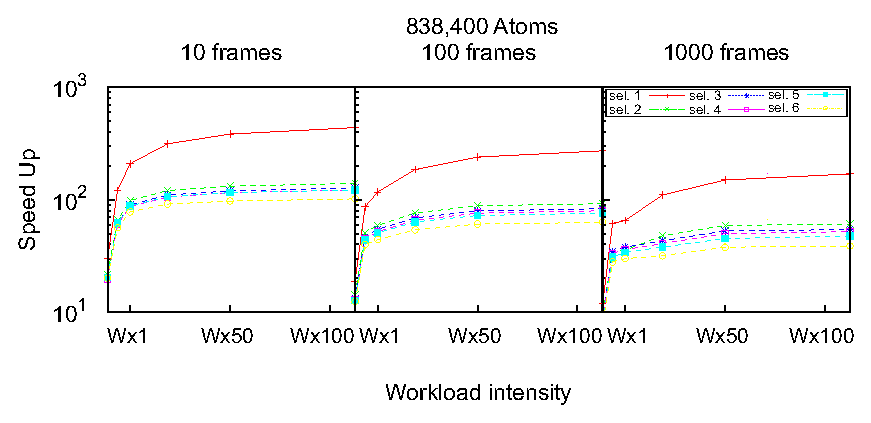
\includegraphics[width=0.5\columnwidth]{images/speedup838K-pomalo-za-4.eps} }
 \caption{ Speed up over different levels of atom selection for 838,400 atoms}
 \label{fg:sample_estimation_old_paper}
\end{figure}

\section{Our approach with improvement}

Reviewing the approach we are coming up with and what it was before helps us analyzing the weak parts and things that we can focus on to eliminate old bottlenecks.

Original non-improvement standard approach with pull-based querying is probably one of the most flexible, because nobody has to think about improvements and complexities, it does it for every chunk of data and pulls it whenever it is needed. As it has already been mentioned, at this point, the biggest challenge is that supposing we have $M$ queries, for $N$ atoms we would have to load every chunk $M$ times for $N$ chunks of data (frames), and apparently it is very time consuming of I/O and non-linear computations, and that is only for linear functions. Improvements could be done on caching level, but again the worst case would be the same complexity, because most of the time there is nothing really to cache, and if there is, it is too big to store it in memory, so, it just has to be re-read from file. Using accumulative data structures and trying to optimize by means of them doesn't help either, because, first of all, it is too big data to store in memory, and, secondly, most of the time it is based on data distribution expectation of some kind, which is not the best solution, because the experiments can be different, thus data distribution is sometimes not predictable (boiling down to a specific physics problem will destroy the abstractness and applicability of the system to variety of other problems and will narrow it down making it less useful). In summary, the bottlenecks in this approach are I/O time consumption and slow data processing (especially for non-linear computation).

After all, push-based system for solution of the given problem is tremendously fast in comparison with pull-based system. General idea is to push a chunk of data (frame) through the pre-defined network of queries that will be needed to run on the data sets, which basically means chunk of data will be read from file and loaded into memory only once in order to go through all the queries. As you can observe \cite{mainPaper}, it can speed up for more than 100 times (depending on workload, number of atoms, and functions being used). It is clear that the biggest challenges in this approach were related to implementation of non-linear functions like SDH, since once the data is pushed through the queries, it is almost not coming back (if it is coming back, the point of optimization is lost), and the idea is to come up with approach to eliminate this overhead and weakness. In this case, it is also important what memory exactly is being used, because trying not to use used parts of the same chunk also matters, because L-level caches of CPU might play a huge role in big data sets. One of the solutions is building quad-tree based data structure that will help optimize the calculation, and it has some expectation from data distribution which can speed up depending on dimensions (2D and 3D). This is a mutual problem of both data loading (memory usage) and its processing, and push-based system is a great approach, because it still remains as an abstract concept applicable to different queries and probably wide variety of other problems of similar kind in different fields.

Finally, we've analyzed some main ideas, advantages, and disadvantages of our approach in this paper which is basically push-based system with optimization on data processing part by means of GPU computation (in other words, parallelism). Reading the data from files is a huge overhead, thus, speedup of push-based system in general is significant over pull-based system in our given case. 
It's been demonstrated in the previous paper with different amount of atoms, frames, and workloads. Since we have to load the data every time there is a different query versus push-based system loads a chunk of data once, it is quite noticeable how the framework contributes to efficiency of analysis of simulation data. You can observe some estimation samples in Figure \ref{fg:sample_estimation_old_paper}. Even though the memory loading and pushing steps are the key features of the proposed design, nevertheless, having general knowledge about the network of queries, in this paper, we will try to focus on optimizing the actual execution of them.

Some of the queries may be very slow due to their nature on a sequential type of computation,  especially, 2-body functions. Since the nature of the data that comes with simulation is basically physical properties of atoms, there is a lot of computation that involves independent primitive mathematical operations, which makes it a perfect problem for parallelism. For example, image processing computations and graphics processing are done on GPUs, because they have a lot of minor primitive independent pixel-based computations.

As it has already been mentioned, although the original idea of push-based system for molecular simulation data analysis was focused on optimizing throughput and usage of loaded data, there were some extra approaches specifically for 2-body functions. For example, Density Map for Spacial Distance Histogram was used in order to avoid additional memory allocation and latency reduction with proven error bounds. SDH is a quite intensive and computational problem, especially with increasing amount of atoms. 

We believe that having this nature of computational problems, the proposed GPU improved version of push-based system will significantly change in terms of performance by incorporating parallelism with CUDA.

%%%%%%%%%%%%%%%%%%%%%%%%%%%%%%%%%%%
%%%%%%%%%%%%%%%%%%%%%%%%%%%%%%%%%%%
\begin{figure}
\centering
\centerline{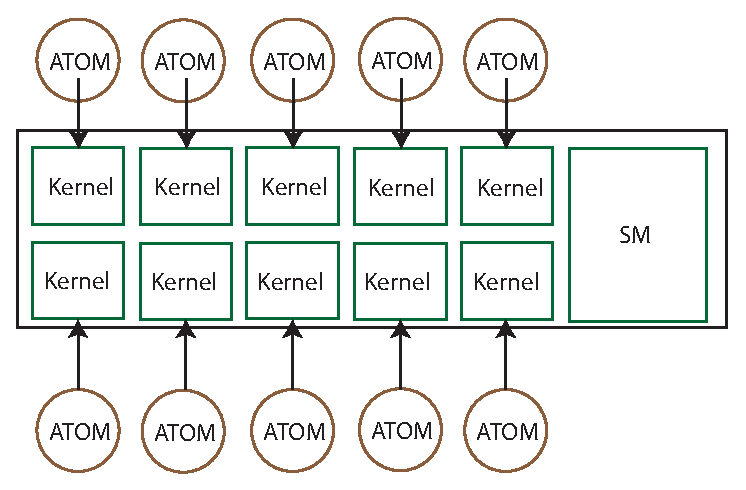
\includegraphics[width=0.5\columnwidth]{images/kernelatom.eps}}
\caption{ Example of atom mapping with kernels}
 \label{fg:kernelatom}


\end{figure}
%%%%%%%%%%%%%%%%%%%%%%%%%%%%%%%%%%%
%%%%%%%%%%%%%%%%%%%%%%%%%%%%%%%%%%%

\section{Contribution and roadmap of the paper} 

In collaboration with Physics Department, the original motivation came from the need of improving analytic query executions performance over big data being generated by simulation software. The idea was to take input stream coming from simulation software (ideally live) and run network of queries very efficiently, because sometimes they might take days and more to compute. The proposed improved version of push-based system for molecular simulation data analysis, we believe, gives an opportunity for scientists to run their analysis fast having an ability to expand network of queries and customize computation functions to get the desired results. 
Our system primarily represents a system that works in several modules that were developed in C, CUDA, Python programming languages that, in combination, give us the desired result to perform efficient computations for the network of queries developed in the previous paper \cite{mainPaper} as well as to prove the concept of optimization of push-based system by means of parallelism with no data loss. We've developed the following modules:

\begin{itemize}
\item[1.] Mock data streamer and generator - tool developed in Python programming language that helps to run performance tests (could also be of other simplest tests like regression) on any kind of data and can be used to simulate random values for physical properties of atoms. The simplest usage of the tool is running a python script with arguments (number of atoms and number of frames).
\item[2.] Main execution script - the main module developed in C and CUDA for the actual computation of the network of queries. Network of queries comes predefined and has to be compiled in the script (though later can be abstracted as a configuration file or argument for interpreting general functions), along with computation implementation function that interact with a given GPU.
\item[3.] Data conversion - this module comes as a part of the code in Main execution script for the users to be able to manipulate data conversion before loading it to GPU. This is for advanced users having capability of optimizing computations and queries on any level of memory hierarchy (CPU and GPU). It is an abstract part which has to be used upon specific cases to optimize specific functions, since there is no way to predict what functions need to be run and how they can be optimized.
\item[4.] Sequential CPU based Push-based system - we re-created original push-based system with the same network of queries as a benchmark for estimation of speedup results of the new approach

\end{itemize}

Taking an advantage of GPU devices nature and incorporating parallelism and streaming for different types of queries, we have come up with a good speed up over sequential processing which gets up to 60 times faster, which is just for sampling with no deep improvements on individual queries (since we believe that it should represent average user usage). Original push-based system already had a good speed up in terms of performance in comparison with original pull-based approach and floats around more than 100 times faster depending on number of atoms, frames, and workload. The module for generation of mock data in Python  was used for benchmarks, and it represents realistic and pessimistic approach of estimation, since there is no data distribution for physical properties values. We believe that it might be quite important, because experiments may vary widely. This mock data has exactly the same information that would come with Gromacs simulation files, and it has exactly the same format as in the previous paper \cite{mainPaper} right before loading it to memory. This improved version has been developed on Amazon Elastic GPU \cite{amazonGPU} nodes that consequently can be replicated and scaled up becoming more of a streaming distributed processing engine (which can be very effective on costs, since it is always easy to scale them up, shut them down and spin them back up), as well as on a simple desktop computer with a GPU device.
In general, major contribution of this paper is the framework of push-based system with an incorporated parallelism based on CUDA programming language. This tool can be integrated into open source project of Gromacs as a custom plugin that can be used for optimized analytic queries to be run over data sets live streaming as well as from files. This will be discussed in more details in further chapters.
The structure of the framework which will be described later is developed in such a way that one can easily add new queries based on their complexity or modify existing ones adding appropriate selections and filters.


%%%%%%%%%%%%%%%%%%%%%%%%%%%%%%%%%%%%%%%%%%%%%%%%%%%%%%%%%%%%%%%%%%%%%%%%%%%%%%%

\chapter{Related Work}\label{sc:relatedwork}

Push-based System for molecular simulation data analysis with its improved GPU features has couple of main focuses in terms of technical implementation and challenges related to those that have already been tried to be solved by other different approaches and software. Here is the review of other works.

\section{Scientific software}

First of all, this system is a tool for scientific computation and in this case particularly for molecular simulation data analysis. PeriScope is a project and initiative by University of Michigan which is a system that will optimize data management for scientific explorations. Relational Database Management Systems were created to optimize business applications and it was revolutionary. Those couldn't be built without these systems with abstract languages like SQL, since it manipulates and automatically takes use of indexes, etc. PeriScope is a project that tries to come up with same approach against scientific data and computation with respectively larger scale.\cite{PeriScope} It is kind of difficult to compare our proposed system with PeriScope, but the original motivation is very similar: optimize scientific computation. PeriScope is a larger project directed towards more abstract solution like RDBMs that would work for any type of data. Another existing tool for scientific data and optimized processing is SciDB. It was created to make scientific data storage and querying better and faster. It is very similar to traditional RDBMS systems in terms of querying language and represent data storage in tables, but states to be faster than Postgres in 2 orders of magnitude. Some of the main features is distributed processing with atomicity and durability (the latter is quite difficult for large scale data), while the disadvantages are no-overwriting (only append mode), single value columns only (no arrays, etc), where records are like simple tuples with join function on querying multiple tables \cite{SciDB}. One of the major differences between Push-based Molecular simulation data analysis tool and the projects above is that our proposed design doesn't do anything with storing the data, because we are mainly concentrating it as a side plugin for processing and querying data in an optimized way, while the actual data generation and storage will be done with the actual simulation software.

\section{Stream processing}
Another major modern issue is live data streaming and live processing, which is also possible with our system. Basically, streaming function is a big challenge and need nowadays, because such networks as Twitter and Facebook are able to keep track of live trends and events, including people's reaction and feedback that have to be reflected real time for tremendous amount of users across the globe. Borealis Stream Processing Software is a tool being developed by MIT, Brown, and Brandeis Universities. It's primary goal is a distributed stream processing and based on Medusa and Aurora. Some of the major functions of the software are highly available distributed large streams processing live, dynamic and highly-scalable with possibility of changing queries live and dynamic vision of query results. \cite{borealis} There is also a similar need in scientific world, since being able to keep track of results in real time might be crucial to be able to make certain explorations. 

As a plugin for optimizing computation of scientific queries against large data sets being produced, Push-based System for Molecular Simulation Data Analysis with GPU improvement should be able to handle data streams as well, in order to get real time results and saving up on time, instead of pulling everything from files later on.

\section{Big Data Frameworks}

We are potentially dealing with data that could easily get up to terabytes and petabytes in sizes, and it will be fair to apply term of big data. Traditional software tools are not able to process Big Data apparently because of huge data sets, thus, special frameworks were developed to handle them. Nowadays there are bunch of frameworks that try to solve this problem. Some of these frameworks are Hadoop \cite{hadoop}, Hadoop with GPU extension \cite{hadoopgpu}, Spark \cite{spark}, Flink \cite{flink} (this is more of a big data stream processing framework) and other ones that are possibly just custom modifications and distributions of these. The mentioned tools help dealing with big data giving an ability to process them in batches on clusters using underlying HDFS (Highly Distributed File System), and normally go along with other utilities that help to apply MapReduce concept. The relationship between our system and this concept along with its implementations is in data sets sizes. Even though we are not using or introducing any non-traditional file systems, in certain scale and problems it could be required, too. In fact, the frameworks listed above could even be used for our problem on top of our system, because, as we discuss in section \ref{sc:conclusion}, it could be extended to a distributed system for analyzing independent frames in parallel. 

\section{GPU and Big Data Processing}
GPU is becoming more popular being used by not only graphics processing, but machine learning, deep learning, search algorithms, sorting, and so on. Having an ability to optimize in tremendous speedups it is being involved in video classifications, natural language processing. Particularly about distributed processing and GPU applications along with it, there has been made some overview and research on what is the current state for common solutions in industry. "There were a lot of custom GPU-Hadoop frameworks after the launch of Mars project. These include C-MR, SteamMR, GPMR, Grex, Panda, Shredder and many others. However, most of these frameworks are no longer supported and were developed for some particular scientific projects. Therefore, a Monte Carlo simulation framework can be hardly applied for a bioinformatics project (say) based on the other algorithms. Moreover, processor technologies are evolving very rapidly. Many new revolutionary architectures have been developed for Sony PlayStation 4, Mali GPU by ARM, Adapteva Multicore Microprocessor etc. Both Mali GPU and Adapteva will be compatible with OpenCL. Xeon Phi co-processor works with OpenCL too, which was launched by INTEL. It has an x86-like architecture and is a 60 core co-processor that supports the PCI Express standard. It consumes just 300watts of energy and provides by giving a performance of 1 TFLOPS in double precision. Tianhe-2 which is the most powerful supercomputer till date implements this co-processor. Though, it is very difficult determine which Processor Computing framework architecture will more robust and high
performance." \cite{hadoopgpu}

Push-based system for MS data analysis is primarily proposing an idea of pushing chunks of data through a network of queries. Essentially, this has also been proposed, as mentioned already, by other frameworks \cite{DataPath,Volcano,Qpipe}. In other words, the major point is to use common data loaded into memory for execution of concurrent queries, which is supposed to eliminate I/O overhead predominantly. The architecture and explanation of DSMS (Data Stream Management System) versus DBMS is well explained in one of the lectures of Morgan and Claypool \cite{DataStreamManagement}. It is very important to capture the differences and specialties of DSMS in network architecture, stream models and windows, scheduling, load balancing, approximation, data expiration, etc, because of the fact that data flow design is the key that required all of those changes to common designs.

Since dealing with data is very delicate in this kind of engines, there are couple of features and requirements that this architecture is applicable to, in order to avoid inappropriate understanding or application of this approach in systems that were covered in the lectures\cite{DataStreamManagement}. The data is volatile and not persistent anymore because of obvious sizes of data.  Since we are pulling the data as little times as possible taking into consideration that MS data is only appended and not modified, the access is sequential rather than random. There are concepts of framing and windowing, and memory is limited in streaming engine, while in DBMS secondary storage is considered to be unlimited. Obviously, because of all of these features or requirements to data, the streaming engine frameworks have some limitations like going back into the history of data, since it is volatile. In fact, this has also been tried by Borealis Streaming Engine \cite{borealis}. On top of the fact that it is a streaming engine, as it was built based on Medusa\cite{medusa} and Aurora\cite{aurora}, it proposes distributed processing at this point having some features to handle errors and look back in the history. In our case, it is primarily a single data source, since it is based on the simulation, though in the future the simulation software systems might introduce distributed computing, too. 

This version of Push-based System of MS data analysis is primarily about taking an advantage of GPU processing of the data. Hadoop is a well-known and well-used framework by many companies nowadays\cite{hadoop}. Its purpose is an ability to store and serve large scale data across clusters in a timely fashion. Since usage of GPU of massive data (not only related to graphics processing) is a relatively new concept, there is also an improved version of Hadoop MapReduce Framework with GPU\cite{hadoopgpu}. Having an ability to scale it up in a distributed computing environment is probably one of the best approaches, but again it might be a bigger overhead in terms of costs, since keeping all nodes up and still being able to solve specific problem sets with hardware stack of a lower capacity raise a will to explore more. Having a specific software for simulation like Gromacs, apparently there is also a possibility of taking an advantage of GPUs. For example, Gromacs allows to optimize simulation and query tools by adding configurations based on GPU device located on the processing computer. Unfortunately, even with this feature, Gromacs doesn't follow push-based approach which means that improvement with GPU with pull data per query makes it negligible.

Gromacs generate output files with physical properties description for each atom in each frame. Modern CPUs do great job in terms of caching and computing, but obviously in this particular problem massive monolithic computation is needed, thus, GPU devices are perfect candidates for such a problem following SIMD type of computation. To be more exact, for example, a single kernel in a GPU device could be dedicated to a single atom (this relationship might change depending on the query, but this is to understand the scale and relationship of multiprocessors), and since we have scientific data of MS, the data is appended, which means that we will only move forward and not take an advantage of caching on chunks high level (though we might take an advantage of GPU caching features particularly in processing phase) having multiple workloads per chunk. Just to make it more clear, workloads in this particular case represent transactions based on number of clients. For example, if we were to serve it all in a streaming fashion, 100 clients might demand concurrent queries with different slight selection properties and expect their results, each workload might be dedicated to each client if not aggregated. Thus, the performance of GPU is certainly increasing based on workload too, which might benefit considerably.


\chapter{Benchmark scientific queries}\label{sc:querynetwork}
Having generated big amount of data in large files, now scientists need to get useful information out of it by means of analysis utilities. Often times, the queries that need to be run over the data look like selection and some kind of accumulation, if it is not more complicated. To be more exact, in this section we will try to summarize common set of queries that were already introduced in the previous work of Push-Based System for Molecular Simulation Data Analysis \cite{mainPaper}. 

In previous work, there has already been developed a network of queries widely used by scientists for MS systems. In Table~\ref{tb:queries} you may observe the common set of queries that has been developed. Basically, these are the queries that need to be improved with our new approach of parallelism. Respectively, $n$, $r_i$, $m_i$, $c_i$ and $q_i$ denote number of particles, coordinates (vector form), mass, charge, and number of electrons of a particle $i$.


\begin{table}[h]
\centering
\resizebox{\columnwidth}{!}
{
\begin{minipage}{\columnwidth}
\centering
\renewcommand*{\arraystretch}{1.5}
\tabcolsep=0.12cm
\begin{tabular}{|c| c|}
\hline %inserts horizontal line
Function Name & Equation/Description \\[0.5ex] 
\hline
Moment of Inertia & $\begin{array} {lcl} I & = & \sum\limits_{i=1}^n m_ir_i \end{array}$ \\[0.5ex]
\hline
Moment of Inertia on z axis & $\begin{array} {lcl} I_z & = & \sum\limits_{i=1}^n m_ir_{zi} \end{array}$ \\[0.5ex]
\hline
Sum of masses & $\begin{array} {lcl} M & = & \sum\limits_{i=1}^n m_i \end{array}$ \\[0.5ex]
\hline
Center of mass & $\begin{array} {lcl} CoM & = & \frac{I}{M} \end{array}$ \\[0.5ex]
\hline
Radius of Gyration & $\begin{array} {lcl} RG & = & \sqrt{\frac{I_z}{M}} \end{array}$ \\[0.5ex]
\hline
Dipole Moment& $\begin{array} {lcl} D & = & \sum\limits_{i=1}^n q_ir_i \end{array}$ \\[0.5ex]
\hline
Dipole Histogram & $\begin{array} {lcl} D_z & = & \sum\limits_{i=1}^n \frac{D}{z} \end{array}$ \\[0.5ex]
\hline
Electron Density & $\begin{array} {lcl} ED & = & \frac{\sum\limits_{i=1}^n (e_i-q_i)}{dz \cdot x \cdot y} \end{array}$ \\[0.5ex]
\hline
Heat Capacity & $\begin{array} {lcl} HC & = & \frac{3000 \cdot \sqrt{T} \cdot boltz}{2 \cdot \sqrt{T}-n \cdot df \cdot VarT} \end{array}$ \\[0.5ex]
\hline
Isothermal Compressibility & $\begin{array} {lcl} I & = & \frac{VarV}{V_{avg} \cdot boltz \cdot T \cdot PresFac} \end{array}$ \\[0.5ex]
\hline
Mean Square Displacement& $\begin{array} {lcl} msd & = & \langle (r_{t+\Delta_t}-r_t)^2 \rangle \end{array}$ \\[0.5ex]
\hline
Diffusion Constant & $\begin{array} {lcl} D_t & = & \frac{6 \cdot msd(t)}{t} \end{array}$ \\[0.5ex]
\hline Velocity Autocorrelation & $\begin{array} {lcl} V_{acor} & =&
\langle (V_{t+\Delta_t}\cdot V_t) \rangle \end{array}$ \\[0.5ex]
\hline
Force Autocorrelation & $\begin{array} {lcl} F_{acor} & = & \langle (F_{t+\Delta_t} \cdot F_t) \rangle \end{array}$ \\[0.5ex]
\hline
Density Function & Histogram of atom counts \\[0.5ex]
\hline
SDH & Histogram of all distances \\[0.5ex]
\hline
RDF & $\begin{array} {lcl} rdf(r) & = & \frac{SDH(r)}{4 \cdot \pi \cdot r^2 \cdot \sigma_r \cdot \rho} \end{array}$ \\[0.5ex]
\hline
\end{tabular}
\caption[Popular analytical queries in MS]{Popular analytical queries in MS }
\label{tb:queries}

\end{minipage}

}
\end{table}

The queries that we consider are related to computations limited within one frame of a molecular simulation. In general, with the given queries we have divided them into two categories: one body functions and multiple body functions. The first ones apparently have linear complexity of $O(n)$, while the other ones have bigger complexity. 

\section{One body functions}
\emph{\textbf{One body functions}} such as sum of masses, center of mass, or simple counting with selection  are of a complexity $O(n)$, thus, in order to get the results for them going through every atom (essentially over the entire data) only once is enough, and taking into consideration the fact that we are going with push-based system, it is done at the same time for all of them.

As you can see in the given table, most of them are basically based on primitive summation or other basic mathematical operations, in our experiments in further sections we will be running result on single precision values or to be more explicit we use float type in C programming language.

\section{Multiple body functions}
\emph{\textbf{Multiple body functions}} such as SDH and RDF (Spacial Distance Histogram and Radial Distribution function) require computation of distances pairwise across all the particles. This is generally combination of two across N data: 	$C\binom{N}{2}$. These are the most expensive queries, thus, it is important to focus on their implementation taking advantage of GPU nature and its processing power. SDH is a very expensive computation, and we have used some of the existing work of ours\cite{sdhgpu} to incorporate in this design.

For computation of histogram it is not enough to visit every value for each atom once, since we have to do pairwise computations, thus it increases complexity of the problem not only computation-wise, but memory-wise as well, which is a bigger concern in our case, since the overhead will be huge and non-linearly relative to the size of data. For this purpose we have come up with a way to optimize the way we use references to memory for each atom, so that we minimize overhead of pulling data all the way from DRAM (GPU).

There might be some dependencies and preliminary computation possibilities. For example, some queries need total mass, and we could compute it before we push it further, but this can be easily done by user based on the complexity and dependency. It is explained in more details in further sections.


\vspace{3mm}
\chapter{The system design}\label{sc:system}
\vspace{3mm}

The proposed design has a pretty straightforward structure which is going to be explained in this section. Shortly, the system starts with original input files (or data) and gets consumed in a sequential manner by simple disk IO framework into random access memory by chunks, then, chunk gets uploaded to GPU device and processed. At some point, the results that need to be shown to the user are transported from global memory of GPU (where they initially get accumulated) to the main memory, and then might get written as well to an output file. General data flow map is represented in Figure  \ref{fg:data-flow}.

\begin{figure}
 \centerline{ 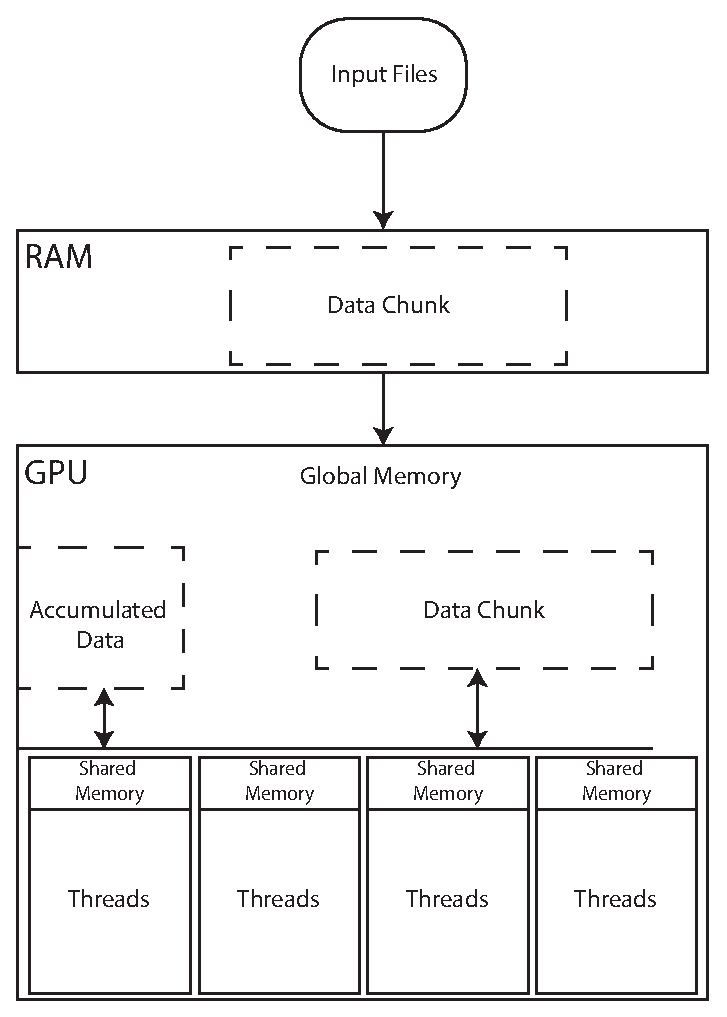
\includegraphics[width=0.65\columnwidth]{images/memory-organization.eps} }
 \caption{Data flow in the improved design of push-based system for MS analysis}
 \label{fg:data-flow}
\end{figure}

\section{Data input}
Since the size of the data in the problem is huge, organization of the data flow is crucial. As mentioned before, original data is retrieved from simulation software output files and in our case it is Gromacs Software's trajectory files\footnote{The file types, their structure, and their decompression has been well explained in the previous paper in section "Data orgranization in main memory"}. For a simulation, there can be several files of different format and usually they are also compressed without any loss of information. Tool for decompressing those files to a flat format for each frame and atom has been developed in the previous work\cite{mainPaper}. 

In order to experiment with different input cases, the input files have been generated with a tool that we have built in Python language. Thus, we are able to generate mock data files with any number of frames and atoms, and the values are random and can be adjusted with needs of the experiment (for example, for cases when we want to analyze bucket widths in a limited space, the coordinates are generated in range of $0 - 1$, etc.). As it has already been mentioned earlier, we don't expect the data to be distributed with a certain behavior, the importance of having this kind of tool to generate mock data is having a variety of random data sets that could reveal any issues related to values provided to the program, on top of that, having the actual file written and then being read has been a part of the experiments to have more realistic use case. In the future, the same script for generating the mock data could be used for regression and performance tests in a distributed implementation of this design as a single source. Potentially input can be technically anything including simple IO sockets that could simply the way the system communicates with other components (f.e. over network) which would also contribute to expanding it to distributed cluster processing (though we believe that it would require additional components such as scheduler or job queues, etc.). To be more exact, the input format of the data and the data represents nothing but a simple array of tuples where each element represents certain descriptor of the given atom in the current frame. We believe that this simple approach makes it a good generalization of solution which would be user friendly for any scientist that wants to run any custom analysis on his data sets.

\section{Data flow architecture}

MS data roughly can be represented as a list of atoms with physical properties aggregated as frames. Thus, we consider a single frame as a chunk which will be loaded into the memory\footnote{Memory in this design might be interpreted differently, since we have a separate device memory on GPUs, but it will be explained better later} and pushed through our network of queries. In this case, it is very convenient, because there are almost no dependencies between frames, rather than list of atoms in the same frame, which potentially again could create additional disk I/O overhead.

Having defined the chunk, we load it from flat format file to RAM. A single atom data structure has all the attributes such as charge, mass, velocity, type of atom, coordinates, and so on. In other words, we have an array of atoms, and most of the attributes (in case of data structure, it is a class field), are simply primitive floats or doubles depending on precision requirements. Next, the same chunk of data with the same structure is loaded onto GPU global memory. GPU devices, in general, have about 4-5 types of memory, and global memory is the biggest and slowest. Consequently, depending on algorithm or query we load parts of data chunk to another types of memory called shared memory. It depends on the actual query, because the same part of chunk can be loaded and unloaded in regards with shared memory several times, especially with SDH.

To summarize, the data goes through several levels of memory hierarchy in our system. Coming as an input from either streaming tool, flat file (our case), or other type of input (f.e. socket) which is either disk memory or RAM it goes to RAM of our system process. After it is loaded to RAM, we continue further and load it to Global Memory of GPU, meanwhile while it is loading the given chunk of data to GPU Global Memory (which happens asynchronously), we as well load the next chunk of data to RAM. In this case, it helps us avoid minor overhead of transferring data between CPU to GPU. Further, we take use of different types of memories in GPU to optimize different queries which will be described in further sections.

\section{Network of queries organization}

Since we assume that our framework should be easily used by a scientist doing MS analysis, it is important to keep queries module as a separate piece of code to make it easily extendable. In order to understand how queries module is organized and the reason for it, we need to understand how CUDA and GPU work.

\emph{\textbf{GPU execution}}. From hardware standpoint, it is important to understand that every GPU device consists of SMs (streaming multiprocessors), and each SM has thousands of registers, which can be partitioned among execution threads. Having this in mind, since this is a pure parallel processing power, the goal is to increase hardware throughput and keep highest utilization to exploit every register given. CUDA is an amazing tool that tries to help developers map this hardware capabilities with the actual application layer. In CUDA we have grids, blocks, and threads, where grid is 3 dimensional unit where each cell is a block, and the same relationship applies between blocks and threads\footnote{This explanation doesn't include memory setup in GPU devices, but it is covered in further sections}. Abstract dimensions given by CUDA are not real entities of physical GPU memory and its organization, but it is just a very convenient way of organizing data and tasks to help GPU scheduler pick and execute the instructions. Originally, this mapping was perfect for solving image processing problems or other graphics computation, since dimensions and such division (e.g. by pixels to threads) is very inherent. As a language feature, in CUDA we have to define such a function called 'kernel' function. Essentially, it is the function where we are supposed to map every execution thread with data and perform the actual execution, this approach is widely known as SIMD\footnote{SIMD - Single Instruction Multiple Data}. As a convenience we have separated one-body functions with multiple-body functions into separate kernels.

\emph{\textbf{One-body queries kernel}}.
Commonly used CUDA array reduction\cite{gpureduction} makes the implementation of all the one-body queries obvious. Figure \ref{fg:reduction} represents general idea of the data mapping, where each cell of the vector can be associated with a thread of execution in the kernel. Having an array of atom data structures, we reduce the array accumulating all the needed data from each atom's attributes. We don't expect much performance improvement from coalesced memory access, since the data structure for atom can eliminate any gain of coalesced memory access, though for specific types of queries it could be possible to aggregate certain attributes into merged arrays and take an advantage of it. In this case, the solution should be simple in order to keep it easily extendable for other simple one-body queries for a scientist to program. We fetch all the atoms from GPU global memory, since we use references to atoms once. In this case, allocating shared memory and copying it over would complicate the implementation and possibly create additional overhead for one time reference usage. Finally, memory transportation and data consumption are implemented for user, thus, he only needs to extend the queries module which consequently can be turned into plugins model.

\emph{\textbf{Two-body queries kernel}}.
SDH (or RDF) is the algorithm that requires special treatment in our design. The point, as mentioned earlier, is that this function requires more than one iteration of the given set of atoms, but rather all combinations of pairs in a given frame, thus, it is not linear complexity. An implementation of this type of query might be very non-intuitive because of the nature of GPUs. Another issue is that since to take an advantage on this type of computation, before writing an implementation for it, a user must have a good understanding of GPU architecture which makes the system less user-friendly. At this point, it is more important to achieve good performance improvement results and then take care of ease of system extensions. As we already mentioned, GPU threads execute in parallel and consume certain amount of work followed by best try of all hardware capacities utilization, but, unfortunately, it is also important to take care of equal workload for every thread independently, so, that utilization is kept high. For this reason, we've come up with a solution that should increase performance of the computation which will be described later.

\begin{figure}
 \centerline{ 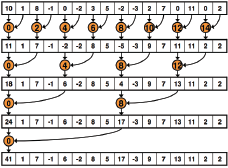
\includegraphics[width=0.65\columnwidth]{images/reduction} }
 \caption{GPU array reduction algorithm sample representation}
 \label{fg:reduction}
\end{figure}

\begin{figure}
 \centerline{ 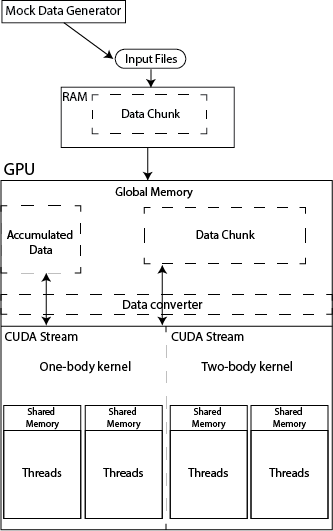
\includegraphics[width=0.65\columnwidth]{images/overallarchitecture} }
 \caption{Overall system architecture}
 \label{fg:overallarchitecture}
\end{figure}


\emph{\textbf{Architecture overview.}}
This section is to emphasize general architecture of the system and summarize the work flow as well as the data flow. In total, we have flat files with ready flat values for each atom aggregated in frames coming into the program as data input using common disk I/O framework of an operating system. Then, once we have loaded a frame (which is considered to be a chunk of the entire data set) onto RAM of our machine, we copy over the entire frame onto the GPU device global memory. It is important that, at this point, we never write any values to simulation files or any other data related to simulation, thus, we don't have to care about any synchronization of incoming data. After this, we have two predefined kernel functions (which were explained before), where first kernel stands for one-body queries, and the second one is for two-body query SDH. Just for architecture clearance and possible future improvements, two kernels are executed in two different streams\footnote{In CUDA stream is another abstract layer of organizing execution threads. They are not guaranteed to be executed at the same time or after each other, GPU scheduling architecture is completely different from CPU having a warp to be single scheduling unit at maximum of 32 threads at a time} (You can see them on Figure\ref{fg:overallarchitecture}). In each kernel we apply certain heuristics to improve memory access using such architecture features of GPU as shared memory and blocking of kernel threads.


\emph{\textbf{GPU grid and block sizes.}} As it has already been mentioned, utilization of hardware on GPU device is important, because it is the key to performance improvement, and the higher utilization is, the bigger improvement is.
The approach we came up with is 1 execution thread per atom. For CUDA version 2.0 maximum number of threads per block is 1024. Blocks are 3 dimensional entities in a 3 dimensional grid. The less abstract unit is, the less overhead we have in communication between them, thus, we try to utilize smallest units more. For example, for 1000,000 atoms, we would allocate 1024 threads per block as a static hard coded value, since we usually have always more than 1024 atoms in simulations. One dimension of grid can take up to 64,000 blocks, thus, if N is bigger than $1024 * 64,000$, than the rest would be allocated to $grid.y$ and $grid.z$ respectively. We have not considered numbers bigger than GPU can allocate, which could be explored in future work. It is important to understand that even though there are abstract entities of grids and blocks, it is not real hardware capacities, but they can affect scheduling and performance consequently. Decision to go with atom to thread execution is because it is pretty convenient to keep high utilization of hardware and still not lose idea if we are about to incorporate more functions, which makes the system more user-friendly, though later on as a plugin we left some room to add data transformer between RAM and GPU global memory, because there are a lot of custom ways to aggregate data and take an advantage of coalesced memory access.

\begin{figure}
 \centerline{ 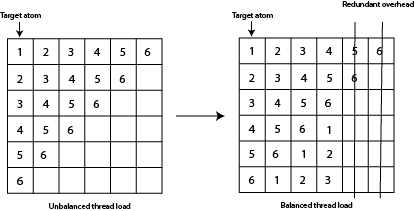
\includegraphics[width=0.5\columnwidth]{images/threadload} }
 \caption{SDH thread loading}
 \label{fg:threadload}
\end{figure}

%%%%%%%%%%%%%%%%%%%%%%%%%%%%%%%%%%%%%%%%%%%%%%%%%%%%%%%%%%%%%%%%%%%%%%%%%%%%%%%


\section{Computation work flow}

Once the data is loaded into global memory of GPU, we have two kernels for two types of queries setup for two different streams. Besides it, we allocate some memory in GPU global memory for results, too, and keep it as an object with fields to easily pull it back when it is ready, in our case all the data sizes are static before the kernels are executed, which follows nature of GPU devices. 


\subsection{One-body functions implementation} 

As it has already been mentioned in previous sections, one body functions are relatively easy to implement, since they don't require iteration through data more than once with a write approach. Our implementation of one-body functions are relatively easy to understand which is what we tried to explain further.

\begin{algorithm}
\caption{One body functions implementation in CPU version}
\label{alg:onebodycpu}
\begin{algorithmic}[1]
\Procedure{OneBodyFuncsCalc}{atoms, atomsCount}
\State \Comment{ $atoms$ is vector of atoms}
\State \Comment{ $atomsCount$ is number of atoms in the frame}

\State $\textit{results} \gets \textit{default initial results value}$

\BState \emph{top}:
\State $\textit{i} \gets \textit{0}$
\State
\While{$i\not=atomsCount$} \Comment{Loop through all the atoms}

\State{$\textit{currentAtom} \gets \textit{atoms[i]}$}
\State
\State{$\textit{calcTotalMass(results, currentAtom)}$}
\State{$\textit{calcTotalCharge(results, currentAtom)}$}
\State{$\textit{calcInertiaX(results, currentAtom)}$}
\State{$\textit{calcInertiaY(results, currentAtom)}$}
\State{$\textit{calcInertiaZ(results, currentAtom)}$}
\State{$\textit{calcDepoleMoment(results, currentAtom)}$}

\State{$\textit{// Here we are adding any other one-body functions}$}

\State
\State $\textit{i} \gets \textit{i + 1}$ \Comment{Increment i}

\EndWhile

\State
\State \textbf{return} $results$ \Comment{Return result for the frame}
\EndProcedure

\State
\Procedure{calcTotalMass}{results, currentAtom} \Comment{Implementation of total mass function}
	\State $results \gets \textit{results.totalmass + currentAtom.mass}$ 
\EndProcedure

\Comment{All other functions}

\end{algorithmic}
\end{algorithm}

\subsubsection{One-body functions implementation in CPU version}

Basically being given a vector of atoms in CPU version implementation (the one that we use for speedup benchmark) we loop through every atom and accumulate all the needed information to RAM. Once we have the result for one-body functions, we take it out for further usage, it can as well be used for further calculations where there are dependencies on such things as total mass, total charge, etc.

We have provided Pseudocode \ref{alg:onebodycpu} of the implementation of one body functions for CPU, which has detailed step-by-step description of the CPU sequential version of push-based system for calculating one-body functions.

\subsubsection{One-body functions implementation in GPU version}

The approach in GPU version of one-body computation code is a lot different, because there are two major changes: the way we deal with the data in memory and mapping of GPU thread kernels to atoms. Both of these approaches drastically change the way we perceive the solution implementation. Basically in the kernel function we assume we've pre-loaded all the needed atoms for current calculations (loading into memory and higher level parts will be described in later sections).

As you can see from the given algorithm (Pseudocode \ref{alg:onebodygpu}), in the thread kernel function it starts with allocation of memory in the block. To be more explicit, every block has its own level of memory called shared memory. To understand the importance of shared memory, it is on-chip memory which can get latency roughly 100x lower than global memory. Further down, we calculate the current index of the atom we need to work with, and this computation takes two lines of code, because we have a grid-based dimensions that have to be flattened back to one-dimension array indexing which was explained in previous sections. Once we are setup, we start accumulating results into the shared memory atomically, because threads within same block might have race condition on write operation. This is one of the reasons why we are doing it locally, because it would also take much more time and overhead to have locks in global memory that would increase race conditions and locking times. After all, we synchronize all threads to make sure that all the records from atoms have been collected to appropriate local results in shared memory. Finally, we collect all the results from blocks' shared memory into global memory in which case it will be much faster, because number of block is not that big. Once a block is finished, first thread of each block will accumulate data from shared memory into global synchronizing the results, every write operation to shared and global memories is atomic (we use native CUDA function atomicAdd which guarantees atomicity). 

\vspace{1cm}

\begin{algorithm}
\caption{Kernel function implementation for one-body queries in GPU}
\label{alg:onebodygpu}
\begin{algorithmic}[1]
\Procedure{gpuonebodyfunctionskernel}{atomsCount, atoms, results}
\State \Comment{ $atoms$ is vector of atoms kept in global gpu memory}
\State \Comment{ $atomsCount$ is number of atoms in the frame kept in global gpu memory}
\State \Comment{ $results$ is number of atoms in the frame kept in global gpu memory}

\BState \emph{top}:

\State $\textit{sdata} \gets \textit{allocate shared memory in each GPU block for fast write access}$ 
\State \Comment{We will use this further to accumulate data across blocks}

\State $\textit{indexX} \gets \textit{blockIdsx.x * blockDim.x + threadIdx.x}$ 
\State \Comment{Identify position of the kernel in the grid scale for coordinate X}
\State $\textit{indexY} \gets \textit{blockIdsx.y * blockDim.y + threadIdx.y}$ 
\State \Comment{Identify position of the kernel in the grid scale for coordinate Y}

\State $\textit{gridWidth} \gets \textit{gridDim.x * blockDim.x}$
\State \Comment{Calculate grid size in kernel units}
\State $\textit{i} \gets \textit{indexY * gridWidth + indexX}$
\State \Comment{Finally get the index of current atom mapped to this kernel}

\State $\textit{sharedResult} \gets \textit{pointer to shared memory head (in this case declared element size as float)}$

\State $\textit{currentAtom} \gets \textit{atoms[i]}$
\State 
\State $\textit{atomicAdd(\&sharedResult[0], currentAtom.mass);}$
\State 
\State $\textit{atomicAdd(\&sharedResult[1], currentAtom.charge);}$
\State $\textit{atomicAdd(\&sharedResult[2], currentAtom.mass * currentAtom.x);}$
\State $\textit{atomicAdd(\&sharedResult[3], currentAtom.mass * currentAtom.y);}$
\State $\textit{atomicAdd(\&sharedResult[3], currentAtom.mass * currentAtom.z);}$
\State $\textit{// other function steps...}$

\State

\State$\textit{// make sure all kernel threads get here and wait for each other}$
\State $\textit{\_\_syncthreads();}$

\State
\State $\textit{// Here we will starting collecting information from each block which will be done by first thread of each block}$
\If {$\textit{threadIdx.x} = 0$}
\State  $\textit{atomicAdd(\&results->mass, sharedResult[0]);}$ \Comment{All atomicAdd functions here are GPU atomic}
\State  $\textit{atomicAdd(\&results->charge, sharedResult[1]);}$
\State  $\textit{atomicAdd(\&results->inertiaX, sharedResult[2]);}$
\State  $\textit{atomicAdd(\&results->inertiaY, sharedResult[3]);}$
\State  $\textit{atomicAdd(\&results->inertiaZ, sharedResult[4]);}$
\State  $\textit{// other functions to accumulate from block shared memory...}$
\EndIf

\State

\EndProcedure

\end{algorithmic}
\end{algorithm}

\subsection{Two-body functions implementation}

Since one of the physical queries is RDF which has underlying SDH calculation, we will describe our approach with SDH for CPU and GPU versions.

\subsubsection{Two-body functions implementation in CPU Version}

Implementation for CPU version of SDH is very simple, we do 2 nested loops that calculate histogram. Since SDH criteria and parameters might vary by bucket width and box size for the simulation space, we've used one sample size for most of them, though results don't change a lot for sequential computation.

\vspace{1cm}

\begin{algorithm}
\caption{SDH in CPU version}
\label{alg:sdhcpu}
\begin{algorithmic}[1]
\Procedure{SDHCPU}{atoms, atomsCount, histogram}

\State $\textit{i} \gets 0$
\While{i < atomsCount}

\State $\textit{j} \gets i + 1$
\While{j < atomsCount}
\State $\textit{dist} \gets calcDistance(atoms[i], atoms[j])$
\State $\textit{Save dist in histogram bucket}$
\State
\State $\textit{j} \gets j + 1$
\EndWhile

\State $\textit{i} \gets i + 1$
\EndWhile

\EndProcedure

\end{algorithmic}
\end{algorithm}



\subsubsection{Two-body functions implementation in GPU Version} 

The approach of solving SDH with GPU is absolutely different just like with one-body queries, though number of computations are the same. We do brute force  $O(\frac{N^2}{2})$ complex solution which is pretty much looking at distance between every pair of atoms. In Pseudocode \ref{alg:sdhgpu} we have tried to provide main logic flow that explains how exactly we implemented kernel for SDH computation. 
Once the first kernel is finished we run the two-body kernel with its own stream. As it has already been mentioned, the bigger workload is in this kernel, because it has higher complexity. GPU streaming multiprocessors are very powerful for straightforward primitive independent calculations, and each core is much weaker than a moden CPU which has a whole bunch of L caches with some prediction behavior systems for code divergence. As you can see on Figure \ref{fg:threadload}, unbalanced thread load assumes for GPU kernel to check every time if the target atom can interact with other atom and if it has to wait till other threads finish their jobs. Thus, we had to come up with a strategy of making equally balanced thread jobs and distribute them among the threads leaving atom to thread mapping as is. 

Here are the main steps of the algorithm:
\begin{itemize}
\item[1.] Get mapped atom
\item[2.] Load all block related atoms to shared memory
\item[3.] Go pairwise with atoms for SDH in a equal balance manner
\item[4.] Synchronize threads
\item[5.] Get everything for results from shared memory to global memory
\end{itemize}


\begin{figure}
 \centerline{ 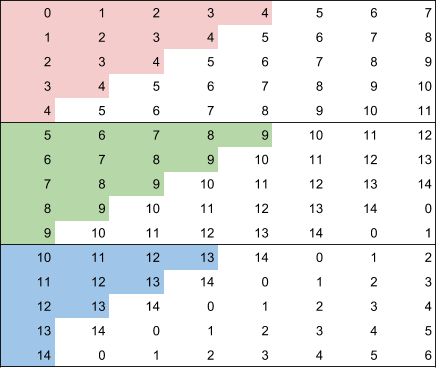
\includegraphics[width=0.5\columnwidth]{images/sharedMem}}
 \caption{Representation of example of shared memory usage}
 \label{fg:sharedMem}
\end{figure}

As we already mentioned, the main purpose of our proposal is the system that allows integration of GPU into push-based system, thus, we didn't go with too sophisticated and optimized implementations for each query that we benchmark, assuming that user's wouldn't do it and having more or less realistic speedup results. Figure \ref{fg:sharedMem} shows swimlanes as execution thread for blocks. Every row is an execution block for an atom, where first element is the mapped atom. First of all, you can observe that we can clearly see that the execution threads are almost equally balanced (exceptions on odd number of atoms) which means that there is no code divergence and low utilization of kernels (no awaiting redundant threads). In this particular example, we have block size 5 with total number of atoms to be 15 (of course, these are just simple examples, realistically it would be millions). Every swimlane (bordered with black) represent within block execution. Secondly, colored numbers are the atoms that we loaded into shared memory. Of course, this is a small improvement, and we can happily add improvement of adding more shared memory and loading as it moves synchronizing threads in the future.

\vspace{1cm}
%%%%%%%%%%%%%%%%%%%%%%%%%
%%%%%      SDH GPU      %%%%%%%%%%%
%%%%%%%%%%%%%%%%%%%%%%%%%
\begin{algorithm}
\caption{Kernel function implementation for SDH in GPU}
\label{alg:sdhgpu}
\begin{algorithmic}[1]
\Procedure{gpusdhkernel}{atomsCount, pdhRes, histogram, atoms, numOfBuckets}

\State $\textit{smem} \gets \textit{pointer to head of SM}$

\State $\textit{sharedHisto} \gets \textit{pointer to the head of smem}$
\State $\textit{sharedAtoms} \gets \textit{pointer to the tail of sharedHisto}$
\State $\textit{index} \gets \textit{calculate index of kernel mapped to this atom}$

\State
\If {$\textit{threadIdx.x} = 0$}

\State $\textit{sharedHisto} \gets \textit{Set all values to 0}$
\State $\textit{start} \gets \textit{index, }
			 \textit{i} \gets \textit{index, }
			 \textit{k} \gets \textit{0,}$
			 
\For {$i < start + blockDim.x$ and $i < atomsCount$}
	\State $\textit{sharedAtoms[k]} \gets \textit{atoms[i]}$
	\Comment{Load local atoms into shared memory}
	\State $\textit{i} \gets \textit{i + 1, } \textit{k} \gets \textit{k + 1}$
\EndFor

\EndIf

\State
\State $\textit{\_\_syncthreads()}$
\State $\textit{threadLoad} = \textit{(atomsCount + 1) / 2}$
\State $\textit{start} \gets \textit{i+1}$
\State $\textit{end} \gets \textit{i + threadLoad, }
\textit{increment end by one if it is odd and total count is even}$

\State $\textit{bi} \gets \textit{blockDim.x * blockIdx.x, } \textit{ei} \gets \textit{bi + blockDim.x}$

\State $\textit{ind1} \gets \textit{threadIdx.x}$

\State $\textit{j} \gets \textit{start}$

\For {$\textit{j} < \textit{end}$}

\State $\textit{ind2} \gets \textit{j mod atomsCount}$
\State $\textit{atom1} \gets \textit{load from shared memory}$

\If{ $\textit{atom2 can be loaded from shared memory}$}
\State $\textit{atom2} \gets \textit{load from local memory}$
\Else
\State $\textit{atom2} \gets \textit{load from global memory}$
\EndIf

\State $\textit{calc distance and atomically write to local histogram}$
\EndFor

\State
\State $\textit{synchronize all threads}$
\State $\textit{gather all histogram from shared into global memory}$
\EndProcedure

\end{algorithmic}
\end{algorithm}



\subsection{Data flow implementation in CPU}

As we have described in earlier sections, our CPU is primarily used for data flow management, triggering of GPU functions, data structure changes, and GPU computation stream manipulations.

\vspace{1cm}
%%%%%%%%%%%%%%%%%%%%%%%%%
%%%%%      CPU FLOW %%%%%%%%%%%
%%%%%%%%%%%%%%%%%%%%%%%%%
\begin{algorithm}
\caption{Main algorithm in CPU for managing data and pushing to GPU}
\label{alg:cpuflow}
\begin{algorithmic}[1]
\Procedure{runsinglekernel}{atomsCount, atoms, workload}

\State $\textit{stream1} \gets \textit{create CUDA stream with cudaStreamCreate}$
\State $\textit{stream2} \gets \textit{create CUDA stream with cudaStreamCreate}$
\State
\State $\textit{gpuResults} \gets \textit{allocate gpu global memory}$
\State $\textit{gpuAtoms} \gets \textit{allocate gpu global memory}$
\State $\textit{gpuHistogram} \gets \textit{allocate gpu global memory}$
\State
\State $\textit{gpuAtoms} \gets \textit{copy atoms from CPU to GPU with cudaMemcpy}$

\State $\textit{gridSize} \gets \textit{compute grid size depending on atom count}$

\State

\For {$workload$}

\State $\textit{gpukernel1(stream1, sharedMemorySize, gpuAtoms, ...)}$
\Comment{One body queries kernel}
\State $\textit{gpukernel2(stream2, sharedMemorySize, gpuAtoms, ...)}$
\Comment{Two body queries kernel}

\State
\State $\textit{cudaStreamSynchronize(stream1)}$
\State $\textit{cudaStreamSynchronize(stream2)}$

\EndFor

\EndProcedure
\end{algorithmic}
\end{algorithm}

\vspace{1cm}

In the Pseudocode \ref{alg:cpuflow} you can see rough logic of our CPU mapping function that primarily allocates all the memory in GPU, triggers kernel function and manipulates streams. This is a prototype which definitely is not the last version, because we can as well avoid overhead of copying data into shared memory while synchronously it will be computing data already contained there. The main steps here are the following. we create to instances of CUDA streams that are again abstract data types that are scheduled by GPU in a special way. We as well allocate memory in GPU for atoms list, histogram results and common results for one-body queries (in this case it is a data structure with fields that represent some accumulated result). Once we are setup with memory management on GPU, we trigger kernel calls one by one each running on a separate CUDA stream. We don't expect them to run really concurrently, because our two kernels are quite heavily loaded, though streaming can definitely be use for memory management optimization.


\vspace{1cm}
%%%%%%%%%%%%%%%%%%%%%%%
%%%%%    CPU FLOW %%%%%%%%%%%
%%%%%%%%%%%%%%%%%%%%%%%
\begin{algorithm}
\caption{Main algorithm in CPU for managing data and pushing to GPU}
\label{alg:cpuflowfuture}
\begin{algorithmic}[1]
\Procedure{runsinglekernel}{atomsCount, atoms, nextAtoms, workload}

\State $\textit{stream1, stream2} \gets \textit{create CUDA stream with cudaStreamCreate}$

\State
\State $\textit{The same routing with allocating memory for now for nextAtoms too}$

\State
\State $\textit{Here we start loading nextAtoms to GPU on stream2 }$
\State

\For {$workload$}

\State $\textit{gpukernel1(stream1, sharedMemorySize, gpuAtoms, ...)}$
\Comment{One body queries kernel}
\State $\textit{gpukernel2(stream1, sharedMemorySize, gpuAtoms, ...)}$
\Comment{Two body queries kernel}

\State
\State $\textit{cudaStreamSynchronize(stream1)}$
\State $\textit{cudaStreamSynchronize(stream2)}$

\EndFor

\EndProcedure
\end{algorithmic}
\end{algorithm}

\vspace{1cm}

The above Pseudocode \ref{alg:cpuflowfuture} shows what memory concurrent could look like. As you can see it is pretty much overlapping $nextAtoms$ loading with computation of $atoms$, which reduces this tiny overhead of copy data over.


%%%%%%%%%%%%%%%%%%%%%%%%%%%%%%%%%%%%%%%%%%%%%%%%%%%%%%%%%%%%%%%%%%%%%%%%%%%%%%%

\chapter{Experiments Results}\label{sc:experiments}

The framework has been developed in a programming language CUDA, and the sequential version for benchmark\cite{mainPaper} has been originally developed in C++. Experiments were run on operating systems which didn't have any additional workload besides usual installation, and the operating systems particularly were Amazon Linux, which doesn't have a lot of modifications except for some additional features for management with Amazon EC-2 Console. We have generated mock data sets with different variations of atoms, frames and ran them with different workloads comparing sequential version of Push-based system with improved version written in CUDA.



\section{Hardware stack}

There are primarily several parts that are really important in this hardware stack. Since this is primarily big data processing, we care about processing power and memory, Of course, things like PCI bus and all the transportation are important as well, but for speedup benchmarks against CPU vs GPU those stay the same for both sides. RAM on the node that we were running has 16GBs. 

\subsection{CPU}
We have summarized main CPU parameters for CPU version and it is described in Table \ref{tb:cpuhardware}. As you may notice, it is a regular server node CPU with 2.60GHz and 3 levels of L cache.

\begin{table}[h!]
	\renewcommand*{\arraystretch}{1.5}
	\tabcolsep=0.12cm
	\centering
  \begin{tabular}{| l | r |}
   \hline
Architecture & x86\_64 \\  \hline
CPU op-mode(s) & 32-bit, 64-bit \\   \hline
Byte Order & Little Endian \\   \hline
CPU(s) & 8 \\   \hline
On-line CPU(s) list & 0-7 \\   \hline
Thread(s) per core & 2 \\   \hline
Core(s) per socket & 4 \\   \hline
CPU family & 6 \\   \hline
Model & 45 \\   \hline
Model name & Intel Xeon E5-2670 2.60GHz \\   \hline
Stepping & 7 \\   \hline
CPU MHz & 2593.814 \\  \hline  
L1d cache & 32K \\   \hline
L1i cache & 32K \\   \hline
L2 cache & 256K \\   \hline
L3 cache & 20480K \\   \hline
NUMA node0 CPU(s) & 0-7 \\  \hline
  \end{tabular}
    \caption{Hardware stack for CPU version of Push-based system benchmark}
      \label{tb:cpuhardware}
\end{table}

\subsection{GPU}

The same CPU has been used for sequential as well as for improved GPU version during experiments with benchmarks. So, for CPU in GPU improved version refer to the same Table \ref{tb:cpuhardware}. For recall, CPU in improved version is used in-between memory loading from file and uploading it to GPU, printing the results to the user, which is not big load. Consequently, we also have GPU device. Hardware summary for GPU device is described in Table \ref{tb:gpuhardware}

\begin{table}[h!]
	\renewcommand*{\arraystretch}{1.5}
	\tabcolsep=0.12cm
  \centering
  \begin{tabular}{| l | r |}
   \hline
	Name & Grid 34C K520 \\ \hline
	Memory & 4095Mib \\ \hline
	Total Nvidia CUDA Cores & 1536 \\ \hline
	Memory Size & 8 GB GDDR5 (4 GB/GPU) \\ \hline
	Total GPUs & 2 GK104 GPUs \\ \hline
  \end{tabular}
    \caption{Hardware stack for GPU version of Push-based system}
    	  \label{tb:gpuhardware}
\end{table}
\section{Data Sets}

As it has already been mentioned, we have developed a small python script that generated data sets that are used for the experiments. It accepts two numbers as arguments (number of atoms and frames respectively) and generate a file with appropriate number of atoms/frames and format. We have generated number of mock data sets in range of $1K-8M$ atoms with $10, 100, 1000$ frames each. For each data set we run workloads with the values: $1, 5, 25, 50, 100$ . Number of atoms and frames are obviously up to the scientist and depend on simulations, but workloads are a bit trickier. First of all, they give us a bit better understanding of the average value, which might vary on different circumstances related to OS, secondly, once this system is integrated into a distributed system, we can imagine that each frame could be processed by a separate node keeping the values inside of the appropriate memory (global or RAM) and generate responses based on the clients selections requests. This possibility will be elaborated in more details in Future Work section.



\emph{\textbf{SDH implementation.}} Even though implementation of SDH can be different, in the previous paper the algorithm in the previous paper was based on quad tree data structure with data proximity approach based on data uniformity\cite{mainPaper}, but in our experiments we follow special CUDA based approach which perfectly fits the nature of GPU devices with the given memory hierarchy, and the number of computations are equal to brute force, consequently, there is no expectation on data uniformity, thus, the problem solution complexity is still the same with the worst case of $O(N^2)$, but processed in parallel by GPU cores. More improvements can be done for acceleration of this approach, but in the system we have not gone too far with data converter module, because initial framework has to be simple and user friendly.

\section{Results}

We have run number of experiments with different number of atoms and frames. Results vary as we choose different data sets, but we can see some tendency towards growth and, fortunately, it is very positive for our improved version of push-based system.

\subsection{Experiment results for 1000 atoms}

Even though we assume that majority of our cases involve huge amount of atoms (starting from hundred thousands), we still ran experiments on smaller amount of atoms to see difference in speedup relatively with the data set sizes. You can observe summary in Figures \ref{fg:exp_1000_10}, \ref{fg:exp_1000_100}, \ref{fg:exp_1000_1000}, \ref{fg:speedup_1000}. There is a minor threshold, where CPU version is faster, where workload is less than 20 on Figure \ref{fg:exp_1000_10}, but it is changed with growth of workload. That presumably is the minor overhead of loading data from CPU to GPU and number of kernels versus computation work actually needs to be done. Once there is more load on computation, strongly GPU accelerates and becomes faster.

\begin{figure}[!tbp]
  \centering
  \begin{minipage}[b]{0.4\textwidth}
    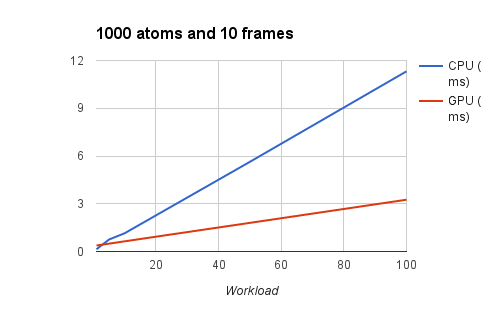
\includegraphics[width=\textwidth]{images/exp_1000_10}
    \caption{Time for 1000 atoms and 10 frames}
    \label{fg:exp_1000_10}
  \end{minipage}
  \hfill
  \begin{minipage}[b]{0.4\textwidth}
    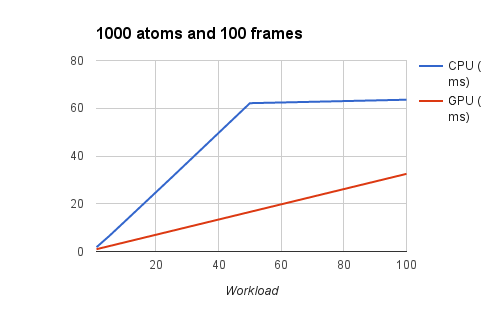
\includegraphics[width=\textwidth]{images/exp_1000_100}
    \caption{Time for 1000 atoms and 100 frames}
     \label{fg:exp_1000_100}
  \end{minipage}
\hfill
  \begin{minipage}[b]{0.4\textwidth}
    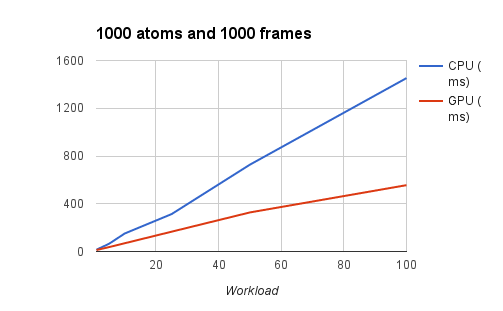
\includegraphics[width=\textwidth]{images/exp_1000_1000}
    \caption{Time for 1000 atoms and 1000 frames}
     \label{fg:exp_1000_1000}
  \end{minipage}
  \hfill
  \begin{minipage}[b]{0.4\textwidth}
    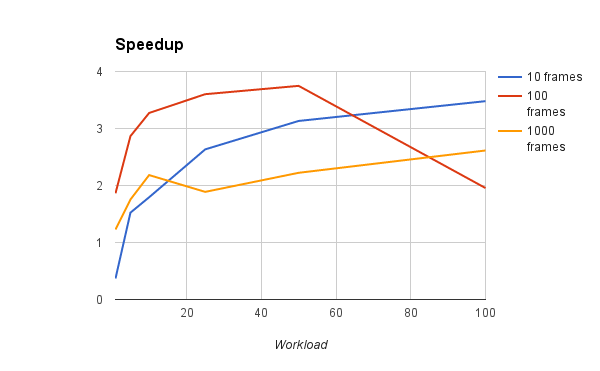
\includegraphics[width=\textwidth]{images/speedup_1000}
    \caption{Speedup for 1000 atoms}
     \label{fg:speedup_1000}
  \end{minipage}
\end{figure}


\vspace{1cm}
\begin{table}[h!]
	\renewcommand*{\arraystretch}{1.5}
	\tabcolsep=0.12cm
  \centering
  \begin{tabular}{| c | c | c | c | c | c |}
   \hline
	Device & Context & Stream & Kernel & Warps Launched & Shared Load \\ \hline
	GRID K520 (0) & 1 & 13 & ${gpu\_one\_body\_function}$ & 32 & 2 \\ \hline
	GRID K520 (0) & 1 & 14 & ${gpu\_two\_body\_function}$ & 32 & 96080 \\ \hline

  \end{tabular}
    \caption{GPU profiling results for 1000 atoms}
    	  \label{tb:gpuprofile1000}
\end{table}

On Table \ref{tb:gpuprofile1000} you can observe results of Nvidia Profiling Tool of how much memory call we did to shared memory for SDH computation. You can also notice that there were 32 warps launched for computing 1000 atoms which is absolutely reasonable, since as we already mentioned one warp (scheduling unit for ultimate parallel execution) has 32 threads maximum, thus ${\frac{1000}{32}}$ \textasciitilde \space$32$. As expected, stream IDs differ for two kernel executions, and both were run on the same GPU device, though we assume that our system can potentially be extended to using multiple GPU devices as well.


%%%%%%%%%%%%%%%%%%%%%%%%%%%%%%%
\subsection{Experiment results for 10,000 atoms}

\begin{figure}[!tbp]
  \centering
  \begin{minipage}[b]{0.4\textwidth}
    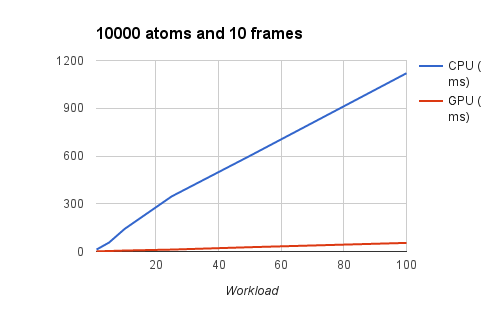
\includegraphics[width=\textwidth]{images/exp_10000_10}
    \caption{Time for 10000 atoms and 10 frames}
    \label{fg:exp_10000_10}
  \end{minipage}
  \hfill
  \begin{minipage}[b]{0.4\textwidth}
    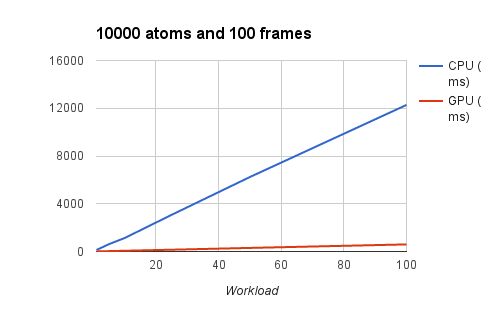
\includegraphics[width=\textwidth]{images/exp_10000_100}
    \caption{Time for 10000 atoms and 100 frames}
     \label{fg:exp_10000_100}
  \end{minipage}
\hfill
  \begin{minipage}[b]{0.4\textwidth}
    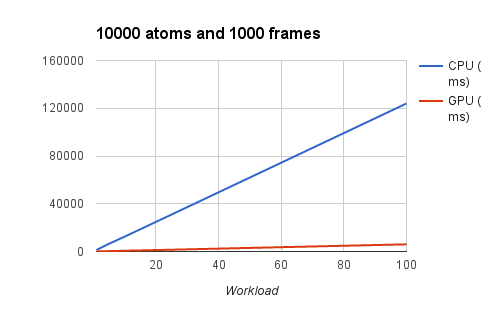
\includegraphics[width=\textwidth]{images/exp_10000_1000}
    \caption{Time for 10000 atoms and 1000 frames}
     \label{fg:exp_10000_1000}
  \end{minipage}
  \hfill
  \begin{minipage}[b]{0.4\textwidth}
    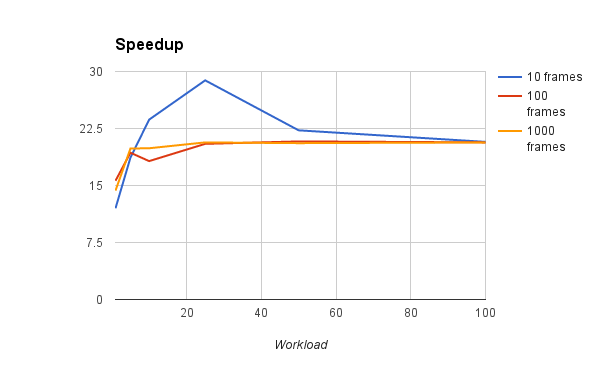
\includegraphics[width=\textwidth]{images/speedup_10000}
    \caption{Speedup for 10000 atoms}
     \label{fg:speedup_10000}
  \end{minipage}
\end{figure}

You can instantly notice that speedup for 1000 atoms is not very impressive, especially for $10$ frames, and the reason for that is nature of GPU and memory transfer. There is a small overhead we have to consider before computing part: in order to let GPU process the data, we have to transfer the data to Global Memory, and upon completion it is needed to load the results back to RAM to show it to the user. In this particular case, for small workload and frames, it is even slower than the sequential processing. Afterwards, the bigger workload the more convincing speedup gets, unfortunately, it doesn't get more than $4$ times for 1000 atoms. Fortunately, scientists usually work with much larger data sets, thus, this doesn't really represent general speedup for average use case.

As you can see, speedup bumps up to almost 30 with 10000 atoms. Once the overhead on memory transfer is covered by computation speedup, it keeps growing. It is important to pay attention to the growth of speedup over growth of workload. It is not that significant, because even though CPUs are much slower, they still use smart caching and internal multi-core processing, which is pretty fast, too, while GPU does pretty straightforward multicore processing, which is the main reason it stagnates.

\subsection{Experiment results for 100,000 atoms}


\begin{figure}[!tbp]
  \centering
  \begin{minipage}[b]{0.4\textwidth}
    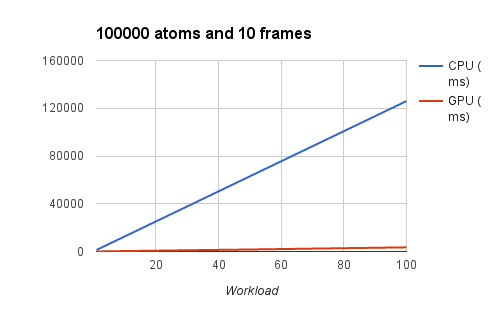
\includegraphics[width=\textwidth]{images/exp_100000_10}
    \caption{Time for 100,000 atoms and 10 frames}
    \label{fg:exp_100000_10}
  \end{minipage}
  \hfill
  \begin{minipage}[b]{0.4\textwidth}
    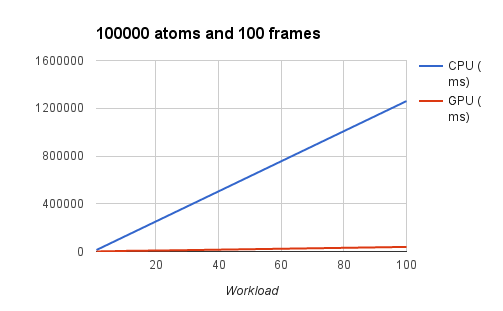
\includegraphics[width=\textwidth]{images/exp_100000_100}
    \caption{Time for 100,000 atoms and 100 frames}
     \label{fg:exp_100000_100}
  \end{minipage}
  \hfill
  \begin{minipage}[b]{0.4\textwidth}
    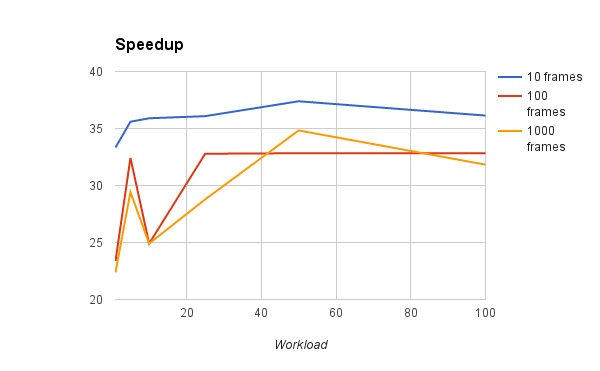
\includegraphics[width=\textwidth]{images/speedup_100000}
    \caption{Speedup for 100,000 atoms}
     \label{fg:speedup_100000}
  \end{minipage}
\end{figure}

When we finally get to the number of atoms that are realistic to the ones scientists use, happily, speedup gets pretty good. Speedup gets up to almost 40 times (Figure \ref{fg:speedup_100000}).

Fortunately, scientific data is much bigger than above examples. You can see average speedup for bigger number of atoms on Figure \ref{fg:chart_max}. The speedup gets upto 70 times which could save huge amount of time for scientists. These results are not the best, as it has been already mentioned earlier, since we have not modified general structure of memory being transferred to Global Memory not taking advantage of coalesced memory access to make it easily extendable. 

\begin{figure}
 \centerline{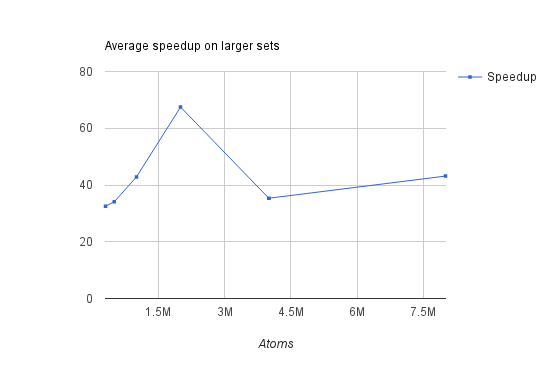
\includegraphics[width=0.5\columnwidth]{images/chart_max}}
 \caption{Speedup for larger number of atoms}
 \label{fg:chart_max}
\end{figure}

It is noticable that growth of the speedup is not stable and with certain number of atoms it drops dramatically. It is because we've used static approach of computing grid dimensions. Besides it, in the future, it can be expanded into a dynamic version that will automatically adjust the grid dimensions choosing least overhead that it has to go with.


\chapter{Conclusions and Future Work}\label{sc:conclusion}
The ultimate goal of this work was to get an improved version of Push-based system for molecular simulation data analysis. As you could see from result on charts (Figure \ref{fg:chart_1000}, \ref{fg:chart_max}), the proposed improved version of the system could save a lot of time for scientists which is up to 60-70 times less of time. The results have been gathered with a single snapshot of the framework tracked in control version system which can be improved with means of data converter module and dynamic grid dimensions computation module. In the future, this system has all potentials to be expanded into a distributed system, where frames could be aggregated by nodes and processed in parallel.\\

%\bibliographystyle{plain}
\bibliographystyle{IEEEtran}
\bibliography{references.bib}
\end{document}

